Este capítulo expõe variadas pesquisas realizadas anteriormente que se assemelham ao presente trabalho e seus principais aspectos.

\section{Robô de Serviço Doméstico Herbert}
Em primeiro lugar, a partir da definição da arquitetura de subsunção e com a orientação do seu criador, Rodney Brooks, \citet{herbert:1988} realizou um experimento para amostrar os princípios dessa arquitetura através da implementação do robô autônomo móvel Herbert.  

O projeto \citet{herbert:1988}  expõe um robô completamente autônomo utilizado em ambientes internos como uma casa, capaz de realizar tarefas de navegação, reconhecimento e manipulação. A sua estrutura física (Figura~\ref{fig:herbert})  é composta por uma base pronta adquirida com o foco na direção do robô, bem como uma parte superior que contém equipamentos de processamento e um braço robótico. 

\begin{figure}[H]
    \centering
    \caption{Estrutura física do Robô Herbert}
    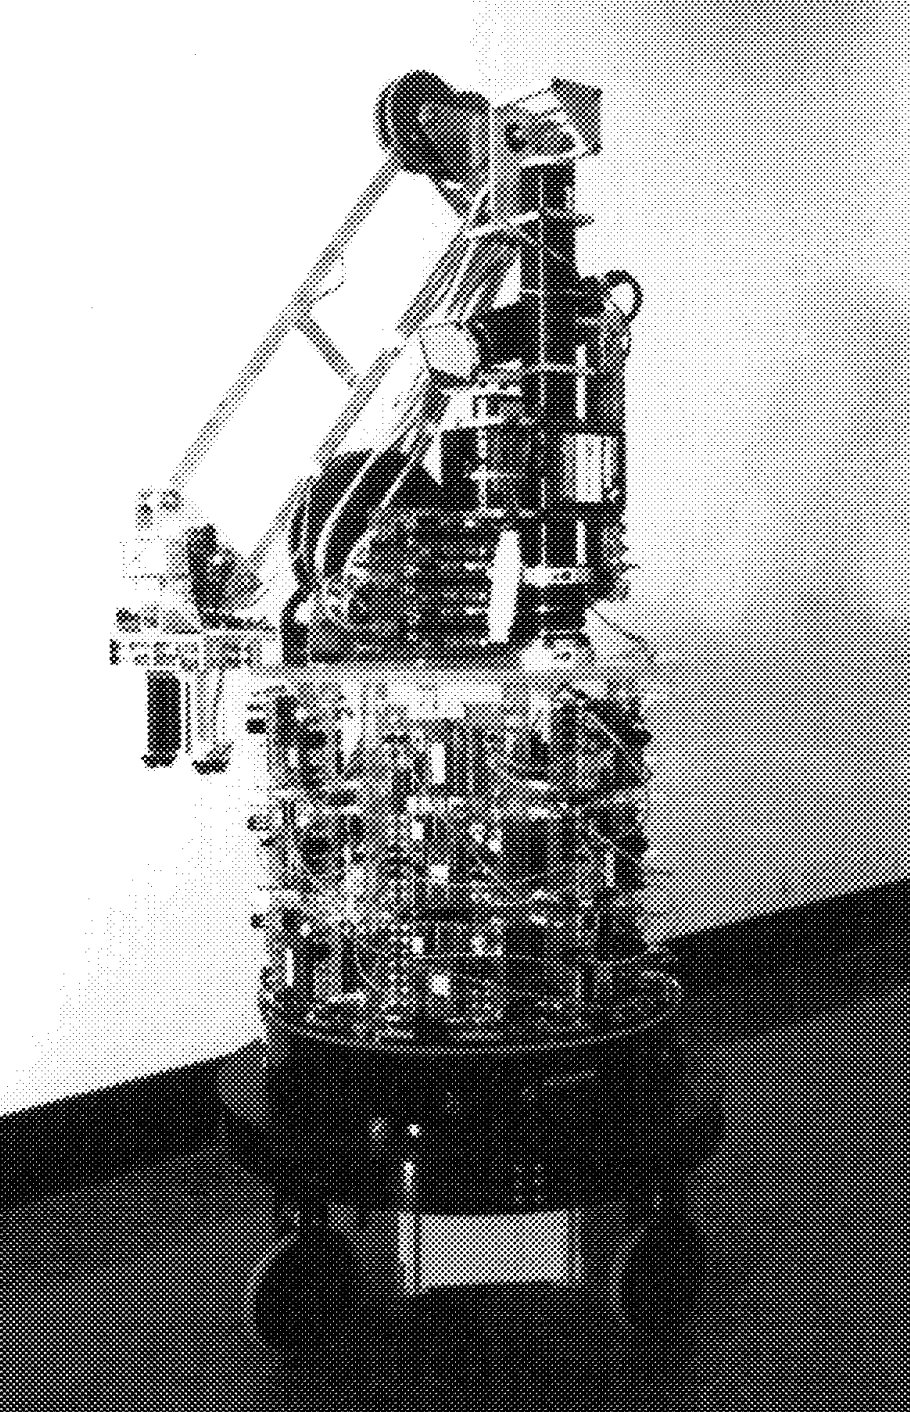
\includegraphics[scale=0.2]{herbert.png}
    \caption*{Fonte: \citet{herbert:1988}.}
    \label{fig:herbert}
\end{figure}

A base do robô Herbert contém a alimentação de energia própria e um computador servo para realizar o mecanismo de direção, o qual atua em um único motor e três rodas. A parte superior do robô é composta por um braço robótico leve e com grau de liberdade suficiente para pegar e soltar objetos no nível do chão e de uma mesa. Essa parte também contém um sensor infravermelho para o robô conseguir se esquivar de obstáculos próximos, fixos ou em movimento, e um sensor scanner de alcance a laser para reconhecimento de objetos. 

Para o controle lógico do robô através da arquitetura de subsunção, foram utilizadas placas com microprocessadores CMOS de 8 bits  que compartilham entre si apenas energia. Para integrar o reconhecimento lógico de objetos com o scanner, foi combinado com o sensor uma árvore de processadores de visão orientada por linha. 

O robô Herbert conseguiu ter um consumo energético baixo para a sua época por ser estruturado por componentes CMOS, além de ter uma resposta mais rápida aos obstáculos por conta do sensor infravermelho que possibilita uma varredura do ambiente em 360 graus. Ademais, sua estrutura foi arranjada de uma maneira que todos seus subsistemas - como as placas de circuitos -  conseguem ser removidas, ajustadas e devolvidas ao corpo do robô com fácil acesso. 

Por ser um projeto realizado no fim dos anos 80, os equipamentos utilizados e as capacidades do robô são limitantes. Apesar de utilizarem processadores com menor custo energético, o dispositivo consegue transitar e realizar suas tarefas pelo ambiente por apenas uma hora. 

Outra desvantagem reconhecida no trabalho é a capacidade do sensor infravermelho em reconhecer a distância de certos objetos conforme o seu tamanho, localização no plano e cor, ou seja, objetos escuros são mais difíceis de serem compreendidos pelo sensor e o mesmo pode se confundir com a profundidade de um objeto pequeno mais próximo e um grande mais longe. Por fim, para realizar todas as tarefas, ao navegar pelo ambiente, o agente armazena as informações de distância e ângulos viajados para conseguir retornar a sua origem depois de cada objeto apanhado para descartá-lo.

\section{Robô de Serviço Doméstico Justina}
Os robôs autônomos de serviço continuaram a ser pesquisados e projetados durante os anos, obtendo avanços notáveis. Similarmente ao robô Herbert, em 2019, foi criado o robô Justina, por \citet{justina:2019}. Este robô emergiu por meio das competições robóticas, conquistando o primeiro lugar no RoboCup@Home de 2019, mostrando o quão crucial essas competições são para o desenvolvimento das tecnologias e motivação da pesquisa na área de robótica, inclusive no tema de robôs de serviço doméstico. 

O equipamento foi produzido pela equipe Pumas, composta por pesquisadores da Universidade de Autonomia Nacional do México. Apesar do time participar constantemente das competições há mais de uma década, sempre buscou aprimorar as tecnologias e conceitos implementados nos seus robôs. Para o RoboCup@Home, mostrou como diferencial um sistema com maior capacidade de compreender a linguagem natural dos comandos de voz dados pelos seres humanos e de manipular objetos com superfícies com menos texturas e geometria mais plana.

O robô Justina (Figura~\ref{fig:justina}) compõe em sua estrutura física uma base com duas rodas onidirecionais, seguida por um torso móvel  metálico capaz de se elevar, dois braços robóticos para a manipulação dos objetos e uma parte superior com suporte do tipo \textit{pan and tilt}. Neste suporte, foi fixado um Kinect da Microsoft e logo acima, um microfone direcional (utilizado para receber os comandos de voz). 

\begin{figure}[H]
    \centering
    \caption{Estrutura física do Robô Justina}
    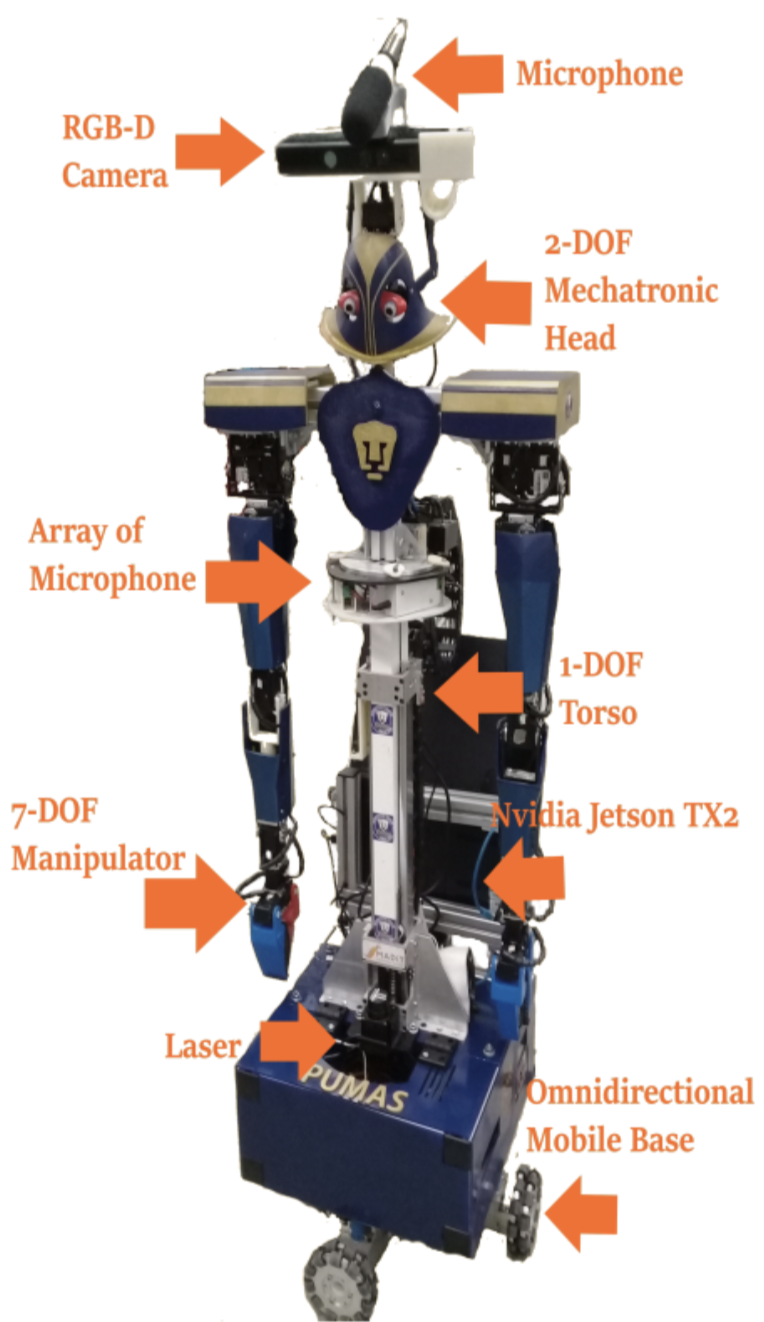
\includegraphics[scale=0.4]{justina.png}
    \caption*{Fonte:\citet{justina:2019}.}
    \label{fig:justina}
\end{figure}

Além da câmera RGB-D do Kinect, são utilizados uma segunda câmera RGB, um laser e quatro microfones para perceber o ambiente onde o robô está inserido. Além disso, como retorno para os seres humanos, foram instaladas caixas de som que emitem uma voz sintetizada informando dados da tarefa em execução. Por fim, para realizar o processamento de imagem obtida a partir das câmeras, foi utilizado um sistema embarcado da NVidia.


O robô da equipe Pumas baseia-se na arquitetura VIRBOT, própria para robôs de serviço domésticos, implementada mediante um conjunto de módulos independentes que executam tarefas próprias e se comunicam entre si. Essa comunicação entre os componentes é realizada pelo sistema operacional de robô (ROS). 

O sistema VIRBOT é composto por quatro camadas nas quais ocorre o processamento das informações externas e internas do robô,  planejamento de objetivos ativados a partir dessas informações, localização do corpo no ambiente por mapas criados pela técnica SLAM e, por fim, a execução das ações e movimentos planejados. De acordo com \citet{justina:2019}, a próxima funcionalidade a ser aprimorada seria deslocamento em todas as direções para melhorar o desempenho da navegação.

\section{TurtleBot3 com SLAM}
No contexto apenas da navegação autônoma, muitas abordagens podem ser utilizadas para resolver o mesmo problema: fazer com que o robô planeje e percorra uma trajetória em um ambiente sem a interferência de humanos. Em \citet{navegacaoSlam:2022} é exposto o uso de SLAM como método eficaz para uma navegação autônoma pelo seu robô Turtlebot3 Burger (Figura~\ref{fig:turtlebotSLAM}). 

\begin{figure}[H]
    \centering
    \caption{Estrutura física do TurtleBot3}
    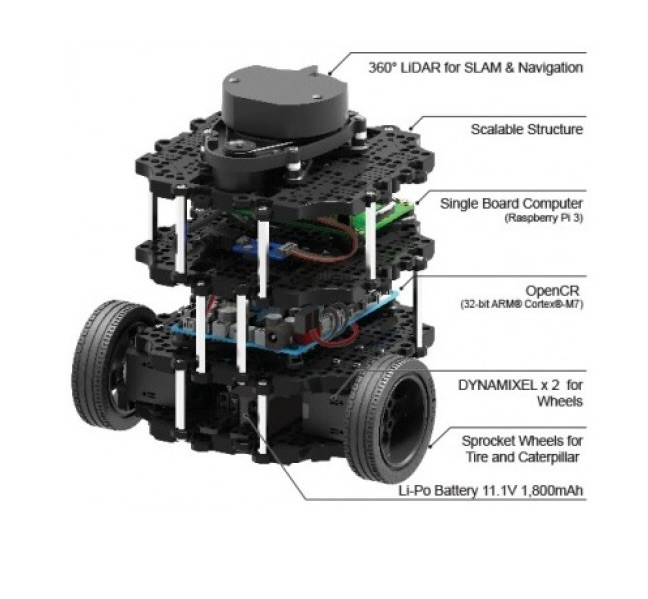
\includegraphics[scale=0.35]{turtlebot3.jpeg}
    \caption*{Fonte:\citet{turtleBot3Burger:2021}.}
    \label{fig:turtlebotSLAM}
\end{figure}

As informações do ambiente foram capturadas por um sensor LiDaR e utilizadas, em conjunto com a odometria  (informação de deslocamento a partir das revoluções das rodas) do robô, no processo SLAM. A fim de melhorar a experiência com a abordagem SLAM, foi utilizado o algoritmo AMCL (\textit{Adaptive Monte Carlo Localization}), sendo uma a versão aprimorada do algoritmo original Localização Monte Carlo. Além disso, o ROS é utilizado como o intermediador entre o sistema, os sensores e o controle lógico (no qual é executado o SLAM adaptado) do Turtlebot3 Burger. 

Visando testar facilmente a solução proposta em comparação com o mapeamento e navegação comum, foi usado o simulador Gazebo. Entretanto, os dois métodos foram testados no mundo real também para assegurar resultados condizentes com a realidade. Com esses experimentos foi apontado que o uso do SLAM aperfeiçoado com o algoritmo de Localização Adaptativa de Monte Carlo tornou a navegação mais resiliente e com maior acurácia.


\section{Robô Autônomo Móvel DPoom}

O desenvolvimento de um robô autônomo móvel, em muitos casos, pode incluir a implementação de recursos que tornam o robô mais custoso, em questão de processamento e preço. Em \citet{dpoom}, seu principal objetivo é diminuir o custo computacional e monetário dos robôs autônomos móveis. Para reduzir o valor da estrutura física do robô, foi utilizada uma câmera RGB-D (capaz de capturar a profundidade dos itens, além da imagem comum colorida) para a percepção do ambiente, ao invés do sensor LiDaR, comumente utilizado e com maior custo. 

Além disso, foi adicionada uma adaptação, menos custosa computacionalmente, do algoritmo clássico de aprendizado por reforço profundo, para evitar obstáculos ao longo da locomoção do seu robô DPoom. Em conjunto, \citet{dpoom} implementou a criação de mapas e posicionamento em tempo real com algoritmo de SLAM integrado a câmera RBG-D. Com isso, foi possível retirar a necessidade da utilização de uma GPU (\textit{Graphic Processing Unit}) e manter o desempenho ideal em tempo real, usufruindo apenas de uma placa-mãe de baixo custo.

A fim de validar seu sistema desenvolvido, \citet{dpoom} integrou todas as funcionalidades com ROS e testou, primeiramente, no simulador Gazebo com uma variação de dez ambientes domésticos estáticos e dinâmicos. O  DPoom (Figura~\ref{fig:dpoom}) também foi testado em ambientes internos reais, com humanos se movimentando ao longo do meio, permitindo validar a interação do robô com as pessoas.

\begin{figure}[h]
    \centering
    \caption{Estrutura física do DPoom}
    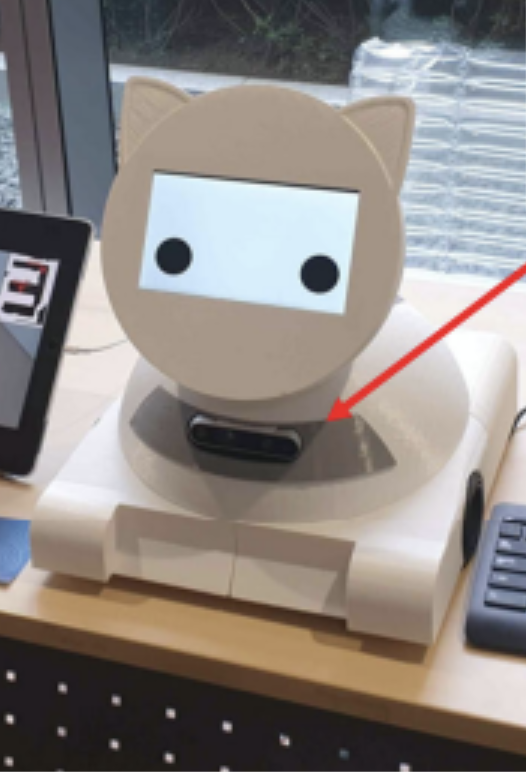
\includegraphics[scale=0.6]{dpoom.png}
    \caption*{Fonte: Adaptado de \citet{dpoom}.}
    \label{fig:dpoom}
\end{figure}

Os principais resultados encontrados em \citet{dpoom} são i) a taxa de operação reduzida,  de apenas 18Hz, para o algoritmo de navegação sem colisão com obstáculos; ii) a taxa baixa de 15\% de colisão; iii) a navegação bem sucedida em ambientes lotados.

\section{Robô Autônomo Móvel com LiDaR e RGB-D}
Em \citet{lidarRGBD},  é proposto um robô autônomo móvel (Figura~\ref{fig:lidarRGBD}) com maior percepção do ambiente, a fim de obter uma navegação mais eficiente ao evitar obstáculos dinâmicos e ser mais seguro a humanos e seus pertences. Para isso, foram implementados, em conjunto, um sensor LiDaR e uma câmera RGB-D para a percepção do ambiente. 

\begin{figure}[H]
    \centering
    \caption{Estrutura física do robô autônomo móvel com LiDaR e RGB-D}
    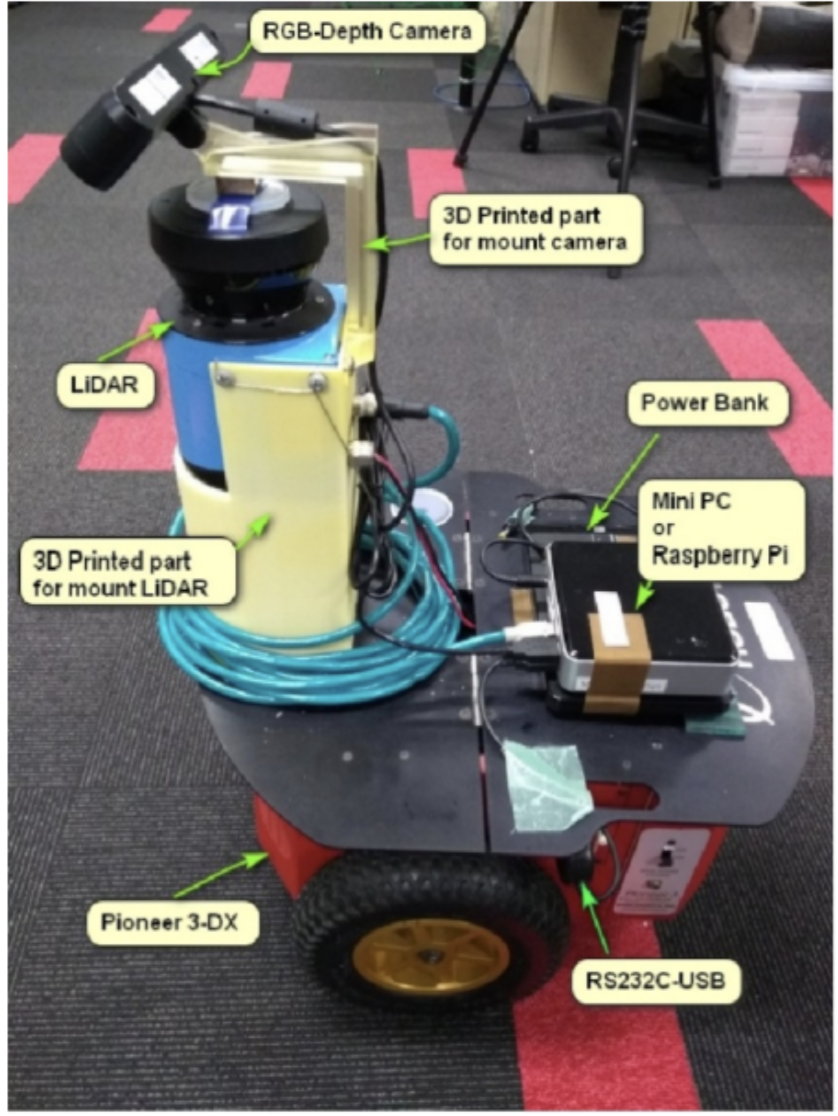
\includegraphics[scale=0.45]{lidarRGBD.png}
    \caption*{Fonte: \citet{lidarRGBD}.}
    \label{fig:lidarRGBD}
\end{figure}

Os instrumentos de percepção acima foram integrados para serem utilizados com o módulo de navegação do sistema ROS. Além disso, \citet{lidarRGBD} implementou uma biblioteca de mapeamento com SLAM do ROS para criar um mapa estático de duas dimensões do ambiente, utilizado em conjunto com o algoritmo AMCL para a localização do robô no ambiente. 

Para analisar o comportamento do robô desenvolvido, \citet{lidarRGBD} testou as suas integrações no simulador Gazebo com diferentes cenários que constituíam de obstáculos em posições e alturas variadas. Com isso, foi possível identificar que a câmera RGB-D permite capturar obstáculos mais altos, mas adiciona um custo de processamento para as informações de profundidade capturadas.

\section{Análise dos Trabalhos Correlatos}

A análise acima de alguns projetos correlatos ao presente trabalho proporcionou um conhecimento mais amplo sobre as possibilidades de implementação de soluções no contexto de robôs de serviço doméstico e navegação autônoma. Com isso, foi possível levantar uma tabela (Tabela~\ref{tab:trabalhosCorrelatos}) com as principais diferenças entre esses projetos conforme as tecnologias implementadas, estrutura física utilizada e considerações finais relevantes ao trabalho em questão. 

\begin{table}[H]
\caption{Principais características dos trabalhos correlatos comparados com AtmosBot}
\label{tab:trabalhosCorrelatos}
\resizebox{\textwidth}{!}{%
\begin{tabular}{p{5cm}|p{5cm}|p{5cm}|p{5cm}}
\multicolumn{1}{c|}{\textbf{Trabalho}} &
  \multicolumn{1}{c|}{\textbf{Principais Tecnologias}} &
  \multicolumn{1}{c|}{\textbf{Estrutura Física}} &
  \multicolumn{1}{c}{\textbf{Considerações Finais}} \\ \hline
Robô Herbert de \citet{herbert:1988} &
  Arquitetura de Subsunção. &
  3 rodas padrão, componentes altamente modularizados, sensor infravermelho e scanner de alcance a laser. &
  Uso de sensor infravermelho impacta negativamente o desempenho. \\ \hline
Robô Justina de \citet{justina:2019} &
  Arquitetura VIRBOT em conjunto com ROS e técnica SLAM para navegação. &
  2 rodas omnidirecionais, câmera Kinect Microsoft, câmera RGB e sensor laser. &
  A locomoção por rodas onidirecionais precisa ser melhorada. \\ \hline
Robô Turtlebot3 Burger de \citet{navegacaoSlam:2022} &
  SLAM aprimorado com Localização Adaptativa de Monte Carlo, em conjunto com ROS. &
  Sensor laser LIDAR. & A navegação é resiliente. \\ \hline
Robô DPoom de \citet{dpoom} &
  Sistema ROS e navegação combinada com SLAM e aprendizado profundo reforçado. &
  Câmera RGB-D. &
  Menos custoso em processamento e recursos. \\ \hline
Robô com LiDaR e RGB-D de \citet{lidarRGBD} &
  SLAM e algoritmo AMCL, integrados com ROS. &
  Sensor LiDaR, câmera RGB-D. & 
  Mais obstáculos capturados, mas maior custo de processamento. \\ \hline
  AtmosBot &
  SLAM com mapeamento simultâneo a exploração e biblioteca de navegação, integrado com ROS e arquitetura de subsunção. &
  Sensor LiDaR e 4 rodas padrão. & 
  Menor custo de processamento e mapeamento menos divergente.
\end{tabular}
%
}
\caption*{Fonte: Autora (2023).}
\end{table}

Diante das informações supracitadas, é possível identificar certas similaridades entre os trabalhos expostos e suas principais diferenças. Assim como no AtmosBot, a abordagem de localização e mapeamento mais utilizado é o SLAM, conforme implantado nos robôs de \citet{justina:2019}, \citet{navegacaoSlam:2022}, \citet{dpoom}, \citet{lidarRGBD}. Para a percepção do ambiente,  os instrumentos mais recorrentes são a câmera RGB e o sensor LiDaR, sendo o último mais utilizado, assim como no AtmosBot. Por fim, a simulação foi utilizada na maioria das pesquisas para a validação parcial ou completa do sistema desenvolvido e os elementos do robô foram integrados pela arquitetura ROS, ambos aspectos presentes no AtmosBot.

As diferenças mais destacáveis entre os trabalhos são os algoritmos mais específicos de localização e de evitar obstáculos, existindo entre eles o AMCL e o aprendizado profundo reforçado. No AtmosBot, nenhum desses algoritmos são utilizados visto que foram implementadas as bibliotecas de navegação do ROS que dispõe o processo de localização sem a necessidade de maiores complementos.

Portanto, a maior contribuição dos trabalhos correlatos analisados é gama de possibilidades existentes para o desenvolvimento de um robô autônomo móvel. Além disso, esses trabalhos expõem as vantagens do uso do ROS, para integrar todos os componentes de navegação, e do programa Gazebo, para realizar as validações necessárias. Essas contribuições são consideradas ao elaborar a proposta da solução, conforme explicado no próximo capítulo que trata sobre o desenvolvimento do modelo proposto.